% L5b student companion deck.
%
% The frame order mirrors the lecture notebook so students can take notes while
% the instructor works through the notebook. The disclaimer is intentionally
% slide 2, by instructor preference.
\documentclass[aspectratio=169,11pt]{beamer}
\usepackage{vnslides}

\newcommand{\Pmeasure}{\mathbb{P}}
\newcommand{\E}{\mathbb{E}}
\newcommand{\Var}{\operatorname{Var}}
\newcommand{\Cov}{\operatorname{Cov}}
\newcommand{\SR}{\operatorname{SR}}
\newcommand{\gbar}{\bar g}
\newcommand{\bA}{\mathbf{A}}
\newcommand{\bC}{\mathbf{C}}
\newcommand{\bZ}{\mathbf{Z}}
\newcommand{\bw}{\mathbf{w}}
\newcommand{\bg}{\mathbf{g}}
\newcommand{\bone}{\mathbf{1}}
\newcommand{\Sig}{\boldsymbol{\Sigma}_{g}}
\newcommand{\Sg}{\hat{\boldsymbol{\Sigma}}_{g}}
\newcommand{\Ch}{\hat{\mathbf{C}}}
\newcommand{\Tan}{\mathcal{T}}

\title{\texorpdfstring{{\vnheavy L5b}}{L5b}: Minimum-Variance Portfolios, the Efficient Frontier, and the Capital Allocation Line}
\subtitle{CHEME 5660 Cornell University}
\author{Copyright Jeffrey Varner 2026. All Rights Reserved}

\begin{document}

\vntitlepage

\begin{frame}{Disclaimer and Risks}
  \vspace{0.6em}
  \textbf{\ink{Training only.}} This content is for training and informational
  purposes only. The teaching team does not make, give, or endorse any offer or
  solicitation to buy or sell securities or derivative products, or provide
  investment or trading advice or strategy.

  \vspace{1.1em}
  \textbf{\ink{Risk.}} Trading involves risk and is generally not recommended for
  those with limited resources, experience, or a low risk tolerance. Past
  performance does not guarantee future success.

  \vspace{1.1em}
  \textbf{\ink{Responsibility.}} You are responsible for your investment decisions
  based on your financial circumstances, objectives, risk tolerance, and
  liquidity needs.
\end{frame}

\begin{frame}{Objectives for Today}
  By the end of this lecture, you should be able to:

  \vspace{0.4em}
  \begin{itemize}\setlength{\itemsep}{0.5em}
    \item \hilite{Formulate portfolio reward and risk}: derive expected growth
      and variance from weighted asset growth rates in matrix form; explain
      diversification through covariance.
    \item \hilite{Construct minimum-variance portfolios}: derive global
      minimum-variance weights by Lagrange multipliers, allowing shorts;
      formulate equality/inequality growth targets, distinguish full and efficient
      frontiers, and explain long-only constraints.
    \item \hilite{Add a risk-free asset}: derive the capital allocation line
      and tangent weights with assumptions; explain Sharpe ratios and two-fund
      separation under borrowing restrictions or unequal lending/borrowing rates.
  \end{itemize}
\end{frame}

\begin{frame}{Lectures and Examples}
  \textbf{\ink{Lecture:}}
  \href{https://github.com/varnerlab/CHEME-5660-CourseRepository-Fall-2026/blob/main/lectures/week-5/L5b/CHEME-5660-L5b-Lecture-MAGBM-Data-Portfolios-Fall-2026.ipynb}{Minimum-Variance Portfolios and the Capital Allocation Line}

  \vspace{0.9em}
  \textbf{\ink{Example 1:}}
  \href{https://github.com/varnerlab/CHEME-5660-CourseRepository-Fall-2026/blob/main/lectures/week-5/L5b/CHEME-5660-L5b-Example-Data-MinVar-Portfolio-Fall-2026.ipynb}{Minimum-Variance Portfolios from Data}

  How do we choose portfolio weights from historical data? We estimate
  inputs from 2014--2024 data, solve the minimum-variance problem, trace the
  frontier and capital allocation line, and compare portfolios using 2025 prices.

  \vspace{0.9em}
  \textbf{\ink{Example 2:}}
  \href{https://github.com/varnerlab/CHEME-5660-CourseRepository-Fall-2026/blob/main/lectures/week-5/L5b/CHEME-5660-L5b-Example-MAGBM-Portfolio-Fall-2026.ipynb}{Portfolio Wealth with Multiple Asset GBM}

  How much might a chosen portfolio's wealth vary? We simulate correlated
  prices and buy-and-hold wealth, compare with 2025 observations, and estimate
  the probability of exceeding a target scaled net present value.
\end{frame}

% ==== concept review =========================================
\begin{frame}{Concept Review: Multiple Asset GBM}
  Recall the multiple asset geometric Brownian motion model from L5a.
  With constant parameters, the price of asset $i=1,\ldots,M$ advances by:
  \[
    S_i(t+\Delta t)=S_i(t)\exp\!\left[
      \mu_{g,i}\Delta t+\sqrt{\Delta t}\,(\bA\bZ)_i\right].
  \]

  Here, $\Delta t>0$ is measured in years, and:
  \begin{itemize}\setlength{\itemsep}{0.6em}
    \item $\mu_{g,i}$ is the asset's \hilite{mean growth rate}
      (year$^{-1}$).
    \item The loading matrix satisfies $\bA\bA^{\top}=\bC$, where
      $\bC$ is the \hilite{covariance rate} (year$^{-1}$).
    \item Use the same vector $\bZ\sim\mathcal N(\mathbf 0,\mathbf I_M)$
      for all assets in a step; draw a new independent vector at each step.
  \end{itemize}
  \vspace{0.5em}
  We estimate the mean growth rates and covariance rate from historical
  growth observations.
\end{frame}

\begin{frame}{Concept Review: Estimating Covariance}
  From $N\ge2$ aligned growth-rate observations, $\bg'$ estimates the mean
  vector $\boldsymbol{\mu}_g$. Subtract each asset's sample mean to form
  $\tilde{\mathbf G}\in\mathbb R^{N\times M}$.

  Recall $\Sig=\bC/\Delta t$. The corresponding estimates are:
  \[
    \boxed{\Sg=\frac{\tilde{\mathbf G}^{\top}\tilde{\mathbf G}}{N-1}},
    \qquad
    \boxed{\Ch=\Delta t\,\Sg}.
  \]

  These estimates have different roles:
  \begin{itemize}\setlength{\itemsep}{0.4em}
    \item Use $\Sg$ to calculate portfolio growth-rate variance
      (year$^{-2}$) and $\Ch$ to simulate prices
      (covariance rate: year$^{-1}$).
    \item The sample covariance is positive semidefinite, so variances are
      nonnegative. Today's closed-form weights require a positive-definite estimate.
  \end{itemize}
  \slidenote{L5a example:}{\href{https://github.com/varnerlab/CHEME-5660-CourseRepository-Fall-2026/blob/main/lectures/week-5/L5a/CHEME-5660-L5a-Example-CovarianceMatrix-Fall-2026.ipynb}{Covariance and Correlation from Data}. Continue here if unfinished.}
\end{frame}

\begin{frame}{Concept Review: Wealth and Scaled NPV}
  Initial weights $w_i\ge0$, with $\sum_iw_i=1$, divide wealth $W_0>0$
  among the assets. Buy $n_i=w_iW_0/S_i(0)$ shares and hold them fixed:
  \[
    \begin{aligned}
      W_t&=W_0\sum_{i=1}^{M}w_i\frac{S_i(t)}{S_i(0)},\\[0.3em]
      \rho_T&=\frac{W_T}{W_0}e^{-g_yT}-1.
    \end{aligned}
  \]
  Here, $g_y$ is the constant benchmark growth rate and $T$ is the holding
  period in years. We allow fractional shares and omit dividends and trading costs.

  \vspace{0.4em}
  Simulated wealth outcomes estimate $\Pmeasure(\rho_T>\rho_\star)$ for a
  target scaled NPV $\rho_\star$.

  \vspace{0.4em}
  L5a sampled candidate allocations. Today, we minimize variance for a
  required expected growth rate.
\end{frame}

% ==== MPT ====================================================
\begin{frame}{Modern Portfolio Theory: Portfolio Reward}
  For $M$ risky assets, $w_i$ is the initial fraction invested in asset $i$,
  with $\sum_iw_i=1$. Hold the weights fixed when calculating reward and risk.
  The model uses weighted growth rates over one observation interval:
  \[
    g_p=\sum_{i=1}^{M}w_i g_i=\bw^{\top}\bg.
  \]

  With fixed weights and $\E[g_i]=\mu_{g,i}$, \hilite{reward} is:
  \[
    \boxed{\E[g_p]=\sum_{i=1}^{M}w_i\E[g_i]
      =\bw^{\top}\boldsymbol{\mu}_g}.
  \]
  From data, $\bw^{\top}\bg'$ estimates expected growth (year$^{-1}$).

  \vspace{0.5em}
  Expected growth is linear in the portfolio weights.
\end{frame}

\begin{frame}{Weighted Growth and Buy-and-Hold Wealth}
  With fixed share counts, one-period wealth and its log growth rate are
  given by:
  \[
    \begin{aligned}
      \frac{W_{\Delta t}}{W_0}
        &=\sum_{i=1}^{M}w_i e^{g_i\Delta t},\\[0.5em]
      \frac{1}{\Delta t}\ln\!\left(\frac{W_{\Delta t}}{W_0}\right)
        &=\frac{1}{\Delta t}\ln\!\left(\sum_{i=1}^{M}w_i e^{g_i\Delta t}\right),
        \qquad W_{\Delta t}>0.
    \end{aligned}
  \]
  The logarithm acts on a sum, so this generally differs from
  $g_p=\sum_iw_i g_i$.

  \vspace{0.5em}
  Use weighted growth rates to choose weights, then use buy-and-hold wealth
  to evaluate the investment through time.

  \vspace{0.5em}
  Next, we measure how the weighted growth rate varies across outcomes.
\end{frame}

\begin{frame}{Modern Portfolio Theory: Portfolio Risk}
  We measure \hilite{risk} by $\Var(g_p)$. With fixed weights and
  covariance matrix $\Sig=\Cov(\bg)$:
  \[
    \boxed{
    \begin{aligned}
      \Var(g_p)
        &=\Cov\!\left(\sum_iw_i g_i,\sum_jw_j g_j\right)\\[0.3em]
        &=\sum_i\sum_jw_iw_j\Cov(g_i,g_j)
        =\bw^{\top}\Sig\bw.
    \end{aligned}}
  \]
  Individual variances (diagonal entries) and pairwise covariances
  (off-diagonal entries) both contribute to risk. From data, use $\Sg$.

  \vspace{0.5em}
  Variance has units year$^{-2}$. Its square root,
  $\sigma_{g,p}=\sqrt{\Var(g_p)}$, is the growth-rate standard deviation
  (year$^{-1}$).

  \vspace{0.5em}
  To see how covariance can reduce risk, consider a two-asset portfolio.
\end{frame}

\begin{frame}{Two-Asset Diversification}
  Invest fractions $w$ and $1-w$, with $0<w<1$, in two assets with positive
  standard deviations $\sigma_{g,1}$ and $\sigma_{g,2}$ and correlation $\rho_{12}$:
  \[
    \Var(g_p)=w^2\sigma_{g,1}^2+(1-w)^2\sigma_{g,2}^2
      +2w(1-w)\rho_{12}\sigma_{g,1}\sigma_{g,2}.
  \]

  Correlation determines what mixing achieves:
  \begin{itemize}\setlength{\itemsep}{0.5em}
    \item At $\rho_{12}=1$, the standard deviation is the weighted average:
      $\sigma_{g,p}=w\sigma_{g,1}+(1-w)\sigma_{g,2}$.
    \item For $\rho_{12}<1$, it falls below that weighted average.
    \item If $\rho_{12}$ is below the smaller standard deviation divided
      by the larger, some allocation has less variance than either asset.
      For 2 and 4 per year, the cutoff is $\rho_{12}<0.5$.
  \end{itemize}

  \vspace{0.4em}
  Positive correlation can still permit diversification.
\end{frame}

\begin{frame}{Growth Rates and Log Returns}
  For an observation interval $\Delta t>0$, asset log returns are
  $\mathbf r=\Delta t\,\bg$. Their weighted average is
  $r_p=\bw^{\top}\mathbf r=\Delta t\,g_p$:
  \[
    \begin{aligned}
      \E[r_p]&=\Delta t\,\E[g_p],\\[0.3em]
      \Var(r_p)&=\Delta t^2\,\Var(g_p).
    \end{aligned}
  \]
  Log returns are dimensionless, with covariance
  $\boldsymbol\Sigma_r=\Delta t^2\Sig$.

  \vspace{0.5em}
  Scaling preserves the optimization problem:
  \begin{itemize}\setlength{\itemsep}{0.5em}
    \item Every portfolio variance is multiplied by the same positive factor
      $\Delta t^2$, preserving the minimizing weights.
    \item Scale the target as $r_\star=\Delta t\,g_\star$ so that the same
      portfolios meet the target.
  \end{itemize}

  \vspace{0.4em}
  Growth rates and log returns therefore give the same optimal weights.
\end{frame}

\begin{frame}{Standard Deviation and Volatility}
  Growth-rate standard deviation depends on the observation interval.
  To calculate volatility, use the covariance rate $\bC=\Delta t\,\Sig$ from L5a:
  \[
    \begin{aligned}
      \sigma_{g,p}&=\sqrt{\bw^{\top}\Sig\bw}
        &&\text{(year$^{-1}$)},\\[0.5em]
      \text{Volatility}&=\sqrt{\bw^{\top}\bC\bw}
        =\sqrt{\Delta t}\,\sigma_{g,p}
        &&\text{(year$^{-1/2}$)}.
    \end{aligned}
  \]

  For daily observations, $\Delta t=1/252$ years:
  \[
    \Ch=\frac{\Sg}{252}.
  \]
  The \hilite{risk axis} in this lecture shows $\sigma_{g,p}$, measured in
  year$^{-1}$.

  \vspace{0.5em}
  With reward and risk defined, we can now choose the weights that minimize
  variance.
\end{frame}

% ==== minimum-variance portfolios ============================
\begin{frame}{The Global Minimum-Variance Portfolio}
  We seek the fully invested portfolio with the smallest growth-rate variance.
  \textbf{Short positions are allowed} ($w_i<0$), and there is
  \textbf{no expected-growth constraint}.
  Assume $\Sig$ is symmetric and positive definite.

  \vspace{0.3em}
  With $\bone\in\mathbb R^M$ the vector of ones, the problem is:
  \[
    \begin{aligned}
      \underset{\bw\in\mathbb R^M}{\text{minimize}}\quad
        &\tfrac12\bw^{\top}\Sig\bw\\
      \text{subject to}\quad &\bone^{\top}\bw=1.
    \end{aligned}
  \]
  The solution and its variance are:
  \[
    \boxed{\bw_{\mathrm{GMV}}
      =\frac{\Sig^{-1}\bone}{\bone^{\top}\Sig^{-1}\bone},
      \qquad \sigma^2_{g,\mathrm{GMV}}
      =\frac{1}{\bone^{\top}\Sig^{-1}\bone}.}
  \]

  The weights depend only on covariance. We now derive this result.
\end{frame}

\begin{frame}{Deriving the GMV Weights}
  Introduce a multiplier $\lambda$ for the budget constraint. The factor
  $1/2$ simplifies the derivative without changing the minimizing weights:
  \[
    \mathcal L(\bw,\lambda)=\tfrac12\bw^{\top}\Sig\bw
      -\lambda(\bone^{\top}\bw-1).
  \]

  \begin{itemize}\setlength{\itemsep}{0.7em}
    \item \textbf{Stationarity:}
      $\Sig\bw-\lambda\bone=\mathbf0$, so
      $\bw=\lambda\Sig^{-1}\bone$.
    \item \textbf{Budget:}
      $1=\lambda\bone^{\top}\Sig^{-1}\bone$, giving
      $\lambda=(\bone^{\top}\Sig^{-1}\bone)^{-1}$.
    \item \textbf{Variance:} use $\Sig\bw=\lambda\bone$ and
      $\bw^{\top}\bone=1$:
      \[
        \sigma^2_{g,\mathrm{GMV}}
          =\bw^{\top}\Sig\bw
          =\lambda\bw^{\top}\bone
          =\lambda
          =\frac{1}{\bone^{\top}\Sig^{-1}\bone}.
      \]
  \end{itemize}

  Positive definiteness makes the objective strictly convex, so these
  weights give the unique minimum.
\end{frame}

\begin{frame}{The Long-Only Problem}
  Long-only weights are nonnegative and sum to one. We also require
  estimated expected growth to reach a \hilite{target floor} $g_\star$
  (year$^{-1}$).

  \vspace{0.4em}
  Using sample means $\bg'$ and estimated covariance $\Sg$, solve:
  \[
    \boxed{
    \begin{aligned}
      \underset{\bw\in\mathbb R^M}{\text{minimize}}\quad
        &\bw^{\top}\Sg\bw\\
      \text{subject to}\quad
        &(\bg')^{\top}\bw\ge g_\star,\\
        &\bone^{\top}\bw=1,\\
        &0\le w_i\le1,\qquad i=1,\ldots,M.
    \end{aligned}}
  \]
  This is a \hilite{convex quadratic program}: the covariance matrix is
  positive semidefinite and the constraints are linear.

  \vspace{0.5em}
  How do these constraints change the solution?
\end{frame}

\begin{frame}{Adding the Portfolio Constraints}
  Use the same estimated inputs and add the restrictions in order:

  \begin{enumerate}\setlength{\itemsep}{0.8em}
    \item \textbf{First, exclude short positions.}
      If the original GMV weights are all nonnegative, keep them.
      Otherwise, solve numerically with $w_i\ge0$ and $\bone^{\top}\bw=1$.
      The result is the \hilite{long-only GMV portfolio}.
    \item \textbf{Then, impose the growth floor.}
      If the long-only GMV portfolio meets $g_\star$, keep its weights.
      For a higher feasible target, solve again; the weights change and
      minimum variance increases.
  \end{enumerate}

  \vspace{0.5em}
  At either step, restricting the portfolio choices cannot lower the
  minimum variance.
\end{frame}

\begin{frame}{The Target-Growth Frontier}
  Allow short positions and require $\bone^{\top}\bw=1$. For each
  \hilite{equality target} $\boldsymbol{\mu}_g^{\top}\bw=g_\star$,
  find the weights with the smallest variance.

  \vspace{0.4em}
  Assume $\Sig$ is positive definite and the asset means are not all equal.
  Define:
  \[
    \begin{aligned}
      a&=\bone^{\top}\Sig^{-1}\bone,
        & b&=\bone^{\top}\Sig^{-1}\boldsymbol{\mu}_g,\\[0.3em]
      c&=\boldsymbol{\mu}_g^{\top}\Sig^{-1}\boldsymbol{\mu}_g,
        & d&=ac-b^2>0.
    \end{aligned}
  \]
  The minimum variance at the target is:
  \[
    \boxed{\sigma_g^2(g_\star)
      =\frac{a g_\star^2-2b g_\star+c}{d}
      =\frac1a+\frac{a}{d}\left(g_\star-\frac ba\right)^2.}
  \]
  Varying $g_\star$ traces the \hilite{minimum-variance frontier}.
  At $g_\star=b/a$, we recover the GMV variance $1/a$; higher or lower
  targets require more variance.
\end{frame}

\begin{frame}{The Efficient Branch}
  A portfolio is efficient if no feasible alternative offers at least as much
  expected growth and no more variance, with one strict improvement.

  \vspace{0.3em}
  \begin{columns}[c]
    \begin{column}{0.59\textwidth}
      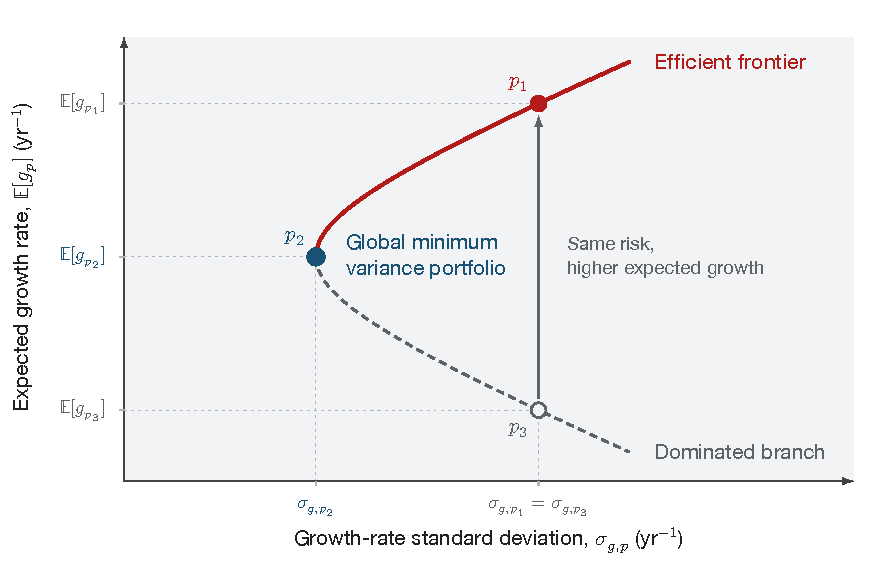
\includegraphics[width=\textwidth]{../figs/minimum-variance-frontier/frontier.pdf}
    \end{column}
    \begin{column}{0.38\textwidth}
      \begin{itemize}\setlength{\itemsep}{0.6em}
        \item $p_2$ is the GMV portfolio.
        \item $p_1$ and $p_3$ have the same risk; $p_1$ has higher growth.
        \item The upper branch, including $p_2$, is efficient.
      \end{itemize}
    \end{column}
  \end{columns}
  \vspace{0.2em}
  Feasible portfolios lie on or to the right of the frontier; moving right adds variance.
\end{frame}

\begin{frame}{Tracing the Long-Only Frontier}
  Long-only portfolio growth is a weighted average of the sample means:
  \[
    \min_i g_i'\ \le\ (\bg')^{\top}\bw\ \le\ \max_i g_i'.
  \]
  This gives a practical target sweep:
  \begin{itemize}\setlength{\itemsep}{0.5em}
    \item Start with $g_\star\le\min_i g_i'$. Every long-only portfolio meets
      the floor, so the solution is the long-only GMV portfolio.
    \item Increase the target to trace the efficient branch. Targets above
      $\max_i g_i'$ are infeasible.
    \item With the same inputs, long-only constraints cannot reduce variance.
      The frontiers meet where the shorts-allowed weights are nonnegative.
  \end{itemize}

  \vspace{0.4em}
  Let's estimate the inputs, sweep the target, and inspect how the weights change.
  \slidenote{Example 1:}{\href{https://github.com/varnerlab/CHEME-5660-CourseRepository-Fall-2026/blob/main/lectures/week-5/L5b/CHEME-5660-L5b-Example-Data-MinVar-Portfolio-Fall-2026.ipynb}{Minimum-Variance Portfolios from Data}}
\end{frame}

% ==== risk-free asset ========================================
\begin{frame}{The Capital Allocation Line}
  A risk-free asset has known growth $g_f$ (year$^{-1}$) and zero variance
  and covariance. A Treasury bill maturing at the holding period's end is
  one example.

  \vspace{0.3em}
  Put fraction $w_f$ in this asset and $1-w_f$ in risky portfolio $p$, with
  $\sigma_{g,p}>0$. The \hilite{complete portfolio} $c$ has:
  \[
    \begin{aligned}
      \E[g_c]&=g_f+(1-w_f)\bigl(\E[g_p]-g_f\bigr),\\[0.3em]
      \sigma_{g,c}&=|1-w_f|\,\sigma_{g,p}.
    \end{aligned}
  \]
  For $w_f\le1$, substitute $1-w_f=\sigma_{g,c}/\sigma_{g,p}$ to obtain the
  \hilite{capital allocation line (CAL)}:
  \[
    \boxed{\E[g_c]=g_f+
      \underbrace{\frac{\E[g_p]-g_f}{\sigma_{g,p}}}_{\text{Sharpe ratio }\SR_p}
      \,\sigma_{g,c}.}
  \]
  Each risky portfolio defines a line through $(0,g_f)$ with slope $\SR_p$.
\end{frame}

\begin{frame}{Which Sharpe Ratio?}
  The CAL slope $\SR_p=(\E[g_p]-g_f)/\sigma_{g,p}$ is dimensionless:
  both numerator and denominator have units year$^{-1}$. It is the Sharpe
  ratio for \hilite{one observation interval}.

  \vspace{0.6em}
  Under independent increments with constant parameters, summing interval
  log returns multiplies the mean by the number of intervals and the
  standard deviation by its square root. For $\tau=1$ year:
  \[
    \boxed{\SR_p^{\mathrm{annual}}
      =\sqrt{\frac{\tau}{\Delta t}}\,\SR_p
      =\frac{\sqrt{\tau}\,(\E[g_p]-g_f)}
        {\sqrt{\bw^{\top}\bC\bw}}.}
  \]
  Daily observations have $\Delta t=1/252$ years, so the annualized ratio is
  $\sqrt{252}\approx15.9$ times the one-day ratio.

  \vspace{0.6em}
  Both conventions rank portfolios identically. L6b onward reports the
  annualized value.
\end{frame}

\begin{frame}{The Tangent Portfolio}
  The \hilite{tangent portfolio} $\Tan$ maximizes the Sharpe ratio and gives
  the steepest CAL. For the closed form, allow shorts, assume $\Sig$ is
  positive definite, and require GMV expected growth to exceed $g_f$.

  \vspace{0.4em}
  Define excess growth $\mathbf e=\boldsymbol{\mu}_g-g_f\bone$.
  Setting the Sharpe-ratio gradient to zero gives:
  \[
    \Sig\bw=\frac{\bw^{\top}\Sig\bw}{\mathbf e^{\top}\bw}\,\mathbf e,
    \qquad \bw\ \propto\ \Sig^{-1}\mathbf e.
  \]
  Normalize the weights to sum to one:
  \[
    \boxed{\bw_{\Tan}
      =\frac{\Sig^{-1}(\boldsymbol{\mu}_g-g_f\bone)}
        {\bone^{\top}\Sig^{-1}(\boldsymbol{\mu}_g-g_f\bone)}.}
  \]
  With long-only weights, solve numerically. The data example approximates
  $\Tan$ by selecting the largest Sharpe ratio along its frontier sweep.
\end{frame}

\begin{frame}{Lending and Borrowing on the CAL}
  \begin{columns}[c]
    \begin{column}{0.63\textwidth}
      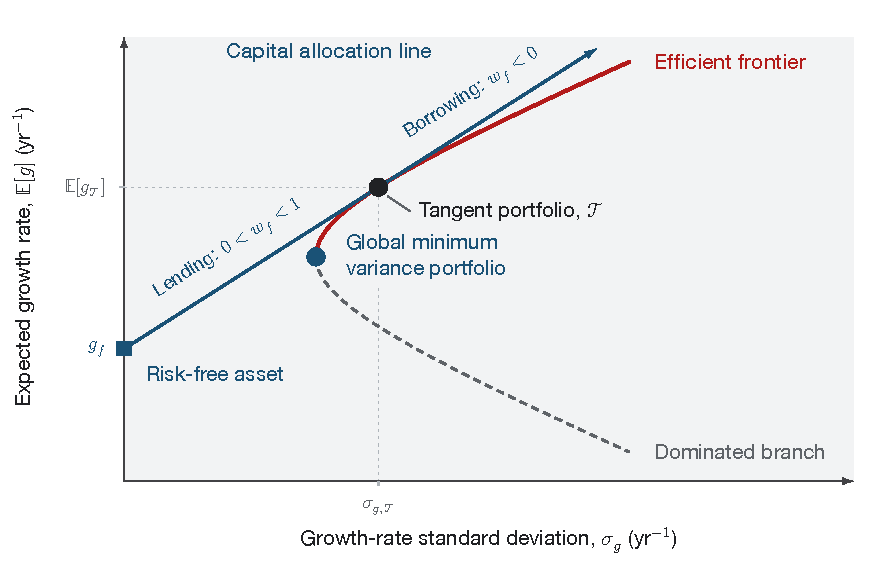
\includegraphics[width=\textwidth]{../figs/capital-allocation-line/cal.pdf}
    \end{column}
    \begin{column}{0.34\textwidth}
      \begin{itemize}\setlength{\itemsep}{0.7em}
        \item \textbf{Lending}, $0<w_f<1$:\newline
          split wealth between the risk-free asset and $\Tan$.
        \item \textbf{Fully risky}, $w_f=0$:\newline
          hold $\Tan$ alone.
        \item \textbf{Borrowing}, $w_f<0$:\newline
          borrow at $g_f$ to invest more in $\Tan$.
      \end{itemize}
    \end{column}
  \end{columns}

  \vspace{0.5em}
  Lending and borrowing use the same rate $g_f$. Changing $w_f$ moves along
  the CAL while keeping the same risky fund.
\end{frame}

\begin{frame}{Two-Fund Separation}
  The two funds are the \hilite{risk-free asset} and the
  \hilite{tangent portfolio} $\Tan$. Investors make two separate choices:

  \begin{enumerate}\setlength{\itemsep}{0.9em}
    \item \textbf{Choose the risky asset mix.}
      Mean-variance investors using the same inputs and investment
      opportunities choose the same $\Tan$, which maximizes the Sharpe ratio.
    \item \textbf{Choose how much to invest in it.}
      Each investor's risk tolerance determines $w_f$, the fraction in the
      risk-free asset. The remaining fraction $1-w_f$ goes into $\Tan$.
  \end{enumerate}

  \vspace{0.6em}
  Risk preferences change the amount invested in $\Tan$; the asset proportions
  within $\Tan$ stay the same.

  \vspace{0.5em}
  This assumes a common rate for lending and borrowing \mbox{(Tobin, 1958)}.
\end{frame}

\begin{frame}{Borrowing and Portfolio Choice}
  With \$100 of our own wealth, a \$150 investment in $\Tan$ requires
  a \$50 loan ($w_f=-0.5$).

  \vspace{0.5em}
  What happens when the borrowing rules change?
  \begin{itemize}\setlength{\itemsep}{0.9em}
    \item \textbf{No borrowing:} the \$150 position is unavailable. We can
      invest at most our \$100 in $\Tan$. To seek more growth than $\Tan$
      offers, we must choose a different risky asset mix.
    \item \textbf{Borrowing costs more than lending earns:} the same \$150
      position has higher financing costs, so it gives less expected net
      growth at the same risk. We must choose the risky mix using that
      borrowing cost.
  \end{itemize}

  \vspace{0.6em}
  Different borrowing opportunities can therefore lead investors to choose
  different risky funds.
\end{frame}

% ==== estimating portfolio inputs =============================
\begin{frame}{Estimating Portfolio Inputs}
  The GMV calculation uses the estimated covariance $\Sg$. The tangent
  calculation also uses the estimated mean growth rates $\bg'$.
  The weights therefore depend on the data and estimation method.

  \begin{itemize}\setlength{\itemsep}{0.8em}
    \item For AMD (2014--2024), mean growth estimates are $0.3120$ per year
      from the sample mean and $0.4397$ per year from L4b's regression:
      a difference of \hilite{12.8 percentage points per year}.
    \item Underestimating an asset combination's variance can make the
      optimizer favor it.
  \end{itemize}

  \vspace{0.5em}
  Our data example evaluates the selected allocations on 2025 prices,
  alongside equal weights and an index fund.

  \vspace{0.5em}
  \slidenote{Example 2:}{\href{https://github.com/varnerlab/CHEME-5660-CourseRepository-Fall-2026/blob/main/lectures/week-5/L5b/CHEME-5660-L5b-Example-MAGBM-Portfolio-Fall-2026.ipynb}{Portfolio Wealth with Multiple Asset GBM}.
    Hold the fitted inputs and allocation fixed; simulate buy-and-hold wealth
    and estimate the probability of exceeding a target scaled NPV.}
\end{frame}

% ==== optional advanced material =============================
\begin{frame}{Optional Advanced Material}
  These examples develop the frontier geometry and input sensitivity further.

  \vspace{0.8em}
  \textbf{\ink{Advanced 1:}}
  \href{https://github.com/varnerlab/CHEME-5660-CourseRepository-Fall-2026/blob/main/lectures/week-5/L5b/advanced/frontier-geometry/CHEME-5660-L5b-Advanced-FrontierGeometry-Fall-2026.ipynb}{Frontier Geometry and the Two-Fund Theorem}

  How can two risky frontier portfolios generate the rest of the curve?
  Derive the weights and vary the mix of two fixed funds. Compare the
  frontier with a 50\% limit on each position's magnitude and with long-only
  weights.

  \vspace{0.8em}
  \textbf{\ink{Advanced 2:}}
  \href{https://github.com/varnerlab/CHEME-5660-CourseRepository-Fall-2026/blob/main/lectures/week-5/L5b/advanced/estimation-risk/CHEME-5660-L5b-Advanced-EstimationRisk-Fall-2026.ipynb}{How Estimates Affect Portfolio Weights}

  How much do weights change when we estimate the inputs again?
  Resample the 2014--2024 observations, vary means and covariance separately,
  and compare GMV and tangent allocations. Evaluate the resulting long-only
  portfolios on the same 2025 prices.
\end{frame}

\begin{frame}{Summary}
  We formulated portfolio reward and risk, constructed minimum-variance
  portfolios, and added a risk-free asset.

  \vspace{0.5em}
  {\large\textbf{\ink{Key takeaways}}}
  \begin{itemize}\setlength{\itemsep}{0.8em}
    \item \hilite{Portfolio reward and risk}: expected growth is linear in the
      weights; variance includes covariance. For two assets with positive
      weights, correlation below one reduces risk below the weighted average
      of their standard deviations.
    \item \hilite{Minimum-variance portfolios}: GMV gives minimum variance
      without a growth constraint. Higher feasible growth targets trace the
      efficient branch; restrictions on the weights change the frontier.
    \item \hilite{The risk-free asset and tangent portfolio}: the CAL slope is
      a Sharpe ratio, maximized by the tangent portfolio. Two-fund separation
      lets investors vary risk through the risk-free allocation.
  \end{itemize}
\end{frame}

\transitionframe{Next: model asset growth using a shared market factor and firm-specific risk.}

\end{document}
